%!TEX TS-program = xelatex
%!TEX encoding = UTF-8 Unicode

\documentclass[galley]{jtlu-article-2col}
\usepackage{tabu}
\renewcommand\query[1]{\relax}

\graphicspath{{../Graphics/},{../../../../jtlugraphics/}}

%% ===== BEGIN ARTICLE DATA BLOCK - FILL IN THIS STUFF ==== %%
%% ===== JTLU publication and copyright info (required) === %%
\jtluissue{1}
\jtluvolume{7}
\jtluyear{2014}
\jtlurights{Robin Lovelace}
\jtluid{nnn}
\setcounter{page}{1}

%% ===== ARTICLE TITLE (required), subtitle (optional) ==== %%
\title{An automated toolset for planning of walking and cycling networks serving specific destinations}
%\subtitle{Subtitle in sentence case}

%% ===== SHORT TITLE (required for page headers) ========== %%
\shorttitle{}

%% ===== AUTHOR INFORMATION (required) ==================== %%
%% Name, affiliation/institution, and email/contact for each
%% Add as many as necessary, separated by "\and":

\author{{\semibfsf Robin Lovelace  } \\University of Leeds  \thanks{r.lovelace@ leeds.ac.uk}
  \and {\bfseries Crispin Cooper} \\University of Cardiff
  % \and {\bfseries } \\
  % \and {\bfseries } \\
}% End authors

%% ===== END ARTICLE DATA BLOCK =========================== %%

\date{} % SET DATE TO NOTHING; NO DATE ON PAPERS

\hypersetup{%
			pdftitle={An automated toolset for planning of walking and cycling networks serving specific destinations},
			pdfauthor={Robin Lovelace},
			pdfproducer={The Journal of Transport and Land Use vol. 7 no. 1 }
			pdfstartpage=1,
			colorlinks=true,
			linkcolor=NavyBlue,
			citecolor=PineGreen,
			urlcolor=BrickRed
} % END HYPERSETUP


% For figures and more when knitting from .Rmd:
% https://stackoverflow.com/questions/41052687/
\providecommand{\tightlist}{%
  \setlength{\itemsep}{0pt}\setlength{\parskip}{0pt}}
\usepackage{longtable,booktabs,array}
\newlength{\cslhangindent}
\setlength{\cslhangindent}{1.5em}
\newlength{\csllabelwidth}
\setlength{\csllabelwidth}{3em}
\newenvironment{CSLReferences}[2] % #1 hanging-ident, #2 entry spacing
 {% don't indent paragraphs
  \setlength{\parindent}{0pt}
  % turn on hanging indent if param 1 is 1
  \ifodd #1 \everypar{\setlength{\hangindent}{\cslhangindent}}\ignorespaces\fi
  % set entry spacing
  \ifnum #2 > 0
  \setlength{\parskip}{#2\baselineskip}
  \fi
 }%
 {}
\usepackage{calc}
\newcommand{\CSLBlock}[1]{#1\hfill\break}
\newcommand{\CSLLeftMargin}[1]{\parbox[t]{\csllabelwidth}{#1}}
\newcommand{\CSLRightInline}[1]{\parbox[t]{\linewidth - \csllabelwidth}{#1}\break}
\newcommand{\CSLIndent}[1]{\hspace{\cslhangindent}#1}

% Custom add-ons
\usepackage[no-math]{fontspec}


\begin{document}
\twocolumn[
\begin{@twocolumnfalse}
\maketitle

\begin{abstract}
Add your article abstract here,
test test test.
lots and lots
and lots and lots
of text\ldots\ldots\ldots\ldots\ldots\ldots\ldots\ldots\ldots\ldots\ldots\ldots.
\end{abstract}

\begin{keywords}
  Keyword 1; keyword 2;
\end{keywords}
\end{@twocolumnfalse}
]
\saythanks

\onecolumn

\hypertarget{introduction}{%
\section{Introduction}\label{introduction}}

There has been much research on mode shift since the origins of applied transport planning and modelling in the 1950s (Boyce and Williams 2015; Aguiléra and Grébert 2014). Within this broad field of research, uptake of `active modes' (walking and cycling) has become a recent focus (Götschi et al. 2017). A range of methods have been used to understand and model walking and cycling levels, with `getting people cycling' being the topic of numerous papers during the 2010 (e.g. Beecham, Wood, and Bowerman 2012; Grisé and El-Geneidy 2018; Larsen, Patterson, and El-Geneidy 2013; Raffler, Brezina, and Emberger 2019; Zhang, Magalhaes, and Wang 2014).
Likewise, getting people walking is worthwhile on environmental (Cervero and Kockelman 1997; Frank and Pivo 1994), community cohesion and health grounds (S. L. Handy 2005; S. L. Handy et al. 2002).
Recently there has been an increase in research activity on various pedestrian models supporting uptake of walking (Aoun 2015; C. H. V. Cooper et al. 2019; Ewing et al. 2014; Griswold et al. 2019; Kuzmyak et al. 2014; Martinez-Gil, Lozano, and Fernández 2017; Munira and Sener 2017; Turner 2017).

Recent policy interest has been shown in planning active transportation networks for specific destinations, such as schools and major employers (Larouche 2015; Uttley and Lovelace 2016).
Encouraging active travel is not just about network infrastructure but complete package of policies, promotion, education, incentives, facilities at destinations (Forsyth and Krizek 2011; S. Handy, van Wee, and Kroesen 2014; McCormack and Shiell 2011; Pucher et al. 2010).
Within this context the specific-destination approach allows for more focused management of the `complete package' as relevant to that destination.
However, modelling active travel potential to specific destinations should not neglect consideration of, and the potential for new infrastructure to integration with, wider walking and cycling networks (Forsyth and Krizek 2011).
It is difficult, in planning practice, to create calibrated models of walking and cycling behaviour, for the following reasons:

\begin{enumerate}
\def\labelenumi{\arabic{enumi}.}
\tightlist
\item
  Models of active modes of transportation are underdeveloped compared to vehicular models
\item
  The small scale of trips makes them sensitive to small scale features of the network. These can include: minor streets (often excluded from vehicle models altogether yet essential for active models); a greater variety of origin/destination points (not only zone centroids or a limited set of representative points within each zone, as with vehicular models); features such as cycle lane, sidewalk and footpath locations and condition, route attractiveness (as measured by e.g.~green vegetation) and street lighting, none of which are reliably mapped.
\item
  The case of cycling suffers from an additional challenge, in that current levels of uptake are low. It is reasonable to assume that as uptake increases, cultural and safety-in-numbers effects may create significant nonlinearity in the response of cycling mode share to cycling infrastructure, as has already happened in e.g.~Holland and Denmark, yet we lack the data to calibrate this (Hollander 2016).
\item
  Reliable, recent local data on mode choice and flows is often not available.
\item
  Finally, the funds invested in construction of active transportation networks --- and hence also in their modelling --- are low compared to typical spending on vehicular networks and their models.
\end{enumerate}

These challenges notwithstanding, two broad approaches to modelling cycling uptake have been particularly prominent in the literature.
The \emph{origin-destination approach} relies on estimates of current travel behaviour, represented in origin-destination datasets reporting the number of trips, e.g.~by mode of travel to work on a typical working day between residential zone origins and workplace destinations. This approach was used in the Propensity to Cycle Tool (PCT), which was originally developed to support strategic cycle network planning based on commuter data for England (Lovelace et al. 2017). The `PCT approach,' which is a particular implementation of the `origin-destination' approach that models cycling uptake in terms of `distance-hilliness decay' functions (which can include other explanatory variables such as traffic levels) has subsequently been adapted to explore cycling potential in other contexts, including cycling uptake in US cities with low cycling levels (Ahmad et al. 2020) and the potential for mode shift to cycling for the `school commute' in across all state schools in England, with publicly available visualisations down to the street level (Goodman et al. 2019).
The PCT has been used by the majority of highway authorities to inform strategic network prioritisation across England (Lovelace, Parkin, and Cohen 2020).\footnote{
  See the `PCT Impact' report (Nov 2020) and many case studies of the use of the PCT in practice at \url{https://www.pct.bike/manual.html}.
  An indication of the level of use of the PCT by local, regional and national government can be obtained by searching for ``propensity to cycle tool'' on web pages hosted on the .gov.uk on services such as \href{https://www.google.com/search?channel=fs\&q=site\%3A.gov.uk+\%22propensity+to+cycle+tool\%22}{Google}.
  At the time of writing the search yielded 814 results, many of which document how the PCT has been used to support Local Cycling and Walking Investment Plans.}
The Rapid Cycleway Prioritisation Tool, which was developed as an extension to the PCT during COVID-19-induced lockdown and subsequent reduction in usage of public transport and peak hour motor traffic to help local authorities prioritise road space reallocation schemes (Lovelace et al. 2020), has also been widely used.\footnote{
  A Department for Transport survey of local authority bids to the Active Travel Fund indicated that 75\% of non-London local authorities used the PCT or Rapid cycleway prioritisation tool to inform and prioritise their proposed schemes (Department for Transport, personal communication).}
The PCT approach is not without limitations:
it omits walking and cannot be used to assess the impacts of existing and potential future infrastructure interventions on mode choice.
Furthermore, detailed origin-destination data is only available from the 10-yearly census, making the data on which the PCT is based increasingly out-of-date.

An alternative approach is to use the topology of the transport network as the basis of modelling using spatial network analysis (SNA) techniques (Chan and Cooper 2019; Crispin H. V. Cooper 2018; J. Cooper and Leahy 2017).
Historically, SNA analysis has been done without origin-destination data, something that can be considered a strength --- because data requirements are reduced --- yet also a weakness: origin-destination data can provide useful information about travel behaviour that networks alone do not reveal.

Within the context of the above challenges, this paper introduces an automated toolchain to assist in production of planning aids for active transportation focused on specific destinations but also highlighting integration with the wider network.
Instead of requiring comprehensive origin-destination data, the approach can leverage single-destination data which is generally available from organizations keen to support active travel planning efforts and more up-to-date then Census data.
The approach was originally developed for Monmouthshire County Council who, like most local authorities across the UK and many local government organisations worldwide, hold data on journeys to public schools and leisure centres. Specific-destination models for cycling were developed using the PCT approach, while specific-destination models for walking were incorporated into the SNA approach.
In addition to showing specific-destination models, however, network-only SNA models are also employed to highlight integration of specific-destination routes with the wider active travel network, the importance of which is highlighted by Forsyth and Krizek (2011).

Considering the challenges associated with accurate prediction and monitoring of walking and cycling mode choice and flows, the aim was not to produce calibrated predictions.
Instead, the aim was to estimate and visualize potential walking and cycling behaviours to support the planning process.
The approach maintains simplicity by deliberately omitting recalibration (the process of updating model results following monitoring): instead it re-uses coefficients describing cycling and walking behaviour calculated in previous research.

As discussed in the final section, the simplicity of the single-destination has several advantages: it keeps modelling costs low, enables transparency of modelling assumptions, and gives users of the outputs the information they need to determine whether unexpected outputs are (a) due to unmet modelling assumptions, or (b) indicative of valid areas of concern in future network plans.
That said, in most cases, modelling outputs showed strong alignment with networks previously planned on the basis of local knowledge.

The approach of automation keeps the expense of deployment realistic for active transportation budgets.
We do so with reproducible methods and open access input data to encourage others to employ the techniques in other areas to support evidence-based interventions to enable cycling uptake and as a basis for future research and development.

\hypertarget{study-area-and-input-data}{%
\section{Study area and input data}\label{study-area-and-input-data}}

The case study area is the local authority district of Monmouthshire, in rural South Wales (Figure \ref{fig:buffers} left).
The research took place in the context of the Active Travel (Wales) Act 2013, which requires local authorities to prepare and submit strategic walking and cycling network plans for approval by the devolved national government (Welsh Government 2020).

\begin{figure}

{\centering 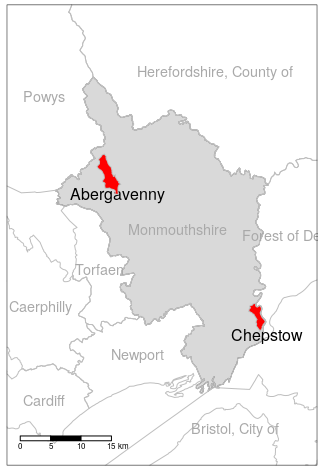
\includegraphics[width=0.4\linewidth,height=10cm]{README_files/figure-gfm/study-area-cropped} 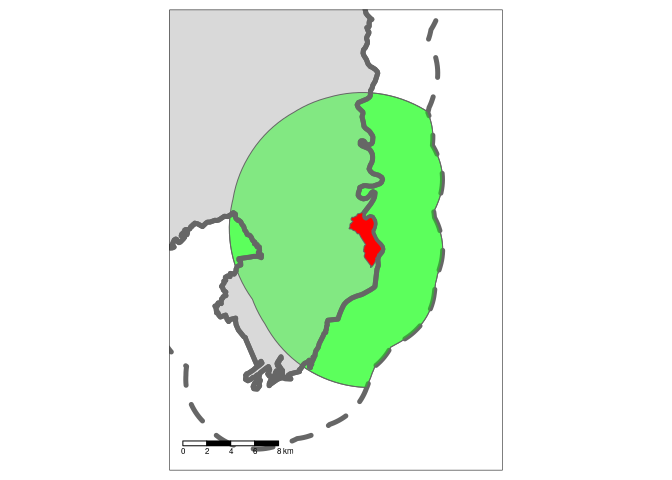
\includegraphics[width=0.5\linewidth,height=10cm]{README_files/figure-latex/buffers-2} 

}

\caption{Illustration of the study area (left) and origin-destination data, represented as desire lines emanating from residential origins with the destination fixed to the destination, simulated from WorldPop data to the destination (right).}\label{fig:buffers}
\end{figure}

The destinations of interest for which travel data was available were schools and leisure centres.
For the purposes of this paper, the locations of these destinations were obtained from OpenStreetMap with the tags (key-value pairs) \texttt{amenity=school} and \texttt{leisure=sports\_centre}.
{[}Add to Figure \ref{fig:buffers} ?{]}

The main input dataset was a list of postcodes associated with each destination which, after being geocoded, were converted into origin-destination (OD) data.
\textbf{{[}Todo, add table showing what this looks like with specific OD pairs linked to a map?{]}}
The other key input was the boundary of the region responsible for the transport system in the local area, available from the UK's official open data web repository data.gov.uk.

Data on approximate locations from which people travel regularly to a particular destination can be obtained from a number of sources, the most reliable being a list of anonymous geocoded addresses or postcodes associated with people who visit each destination regularly.
In cases where such datasets, derived from routine databases surveys or official/commercial records, are missing, they can be simulated using a range of techniques.
For the purposes of this paper, records of the number of people travelling from each postcode to each destination is confidential.
To enable full reproducibility to demonstrate the methods, we simulate origins using WorldPop data (Tatem 2017), resulting in desire lines illustrated in Figure \ref{fig:buffers} right.\footnote{
  For accuracy we recommend using real not simulated data where available.}

The other key input, for spatial network analysis, is route network data.
This can be obtained from OpenStreetMap, which has global coverage (although quality varies).
The OSM data for the study area is represented in Figure \ref{fig:osminput}.
Terrain data was included by draping the OSM network over a digital elevation model constructed from the open licensed Ordnance Survey Terrain 50 data (open access digital elevation data is available for most places, although not at the 50 m resolution used in this study).

\begin{figure}

{\centering 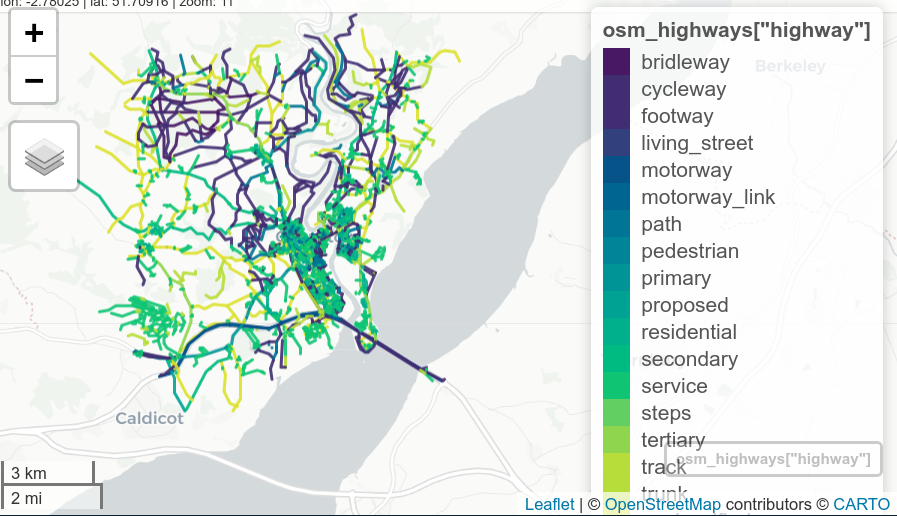
\includegraphics[width=0.5\linewidth]{figures/osm-infra-chepstow} 

}

\caption{OSM data for the study area (placeholder - RL to update)}\label{fig:osminput}
\end{figure}

\hypertarget{methods}{%
\section{Methods}\label{methods}}

Figure \ref{fig:flowchart} shows a summary of the modelling layers output from our toolchain; these are described in greater detail below.
Feedback from planners indicated a need for a simplified set of outputs, therefore we also identified key layers to be included in two summaries (one for walking, one for cycling) --- key layers are identified in red in Figure \ref{fig:flowchart}.

\begin{figure}

{\centering 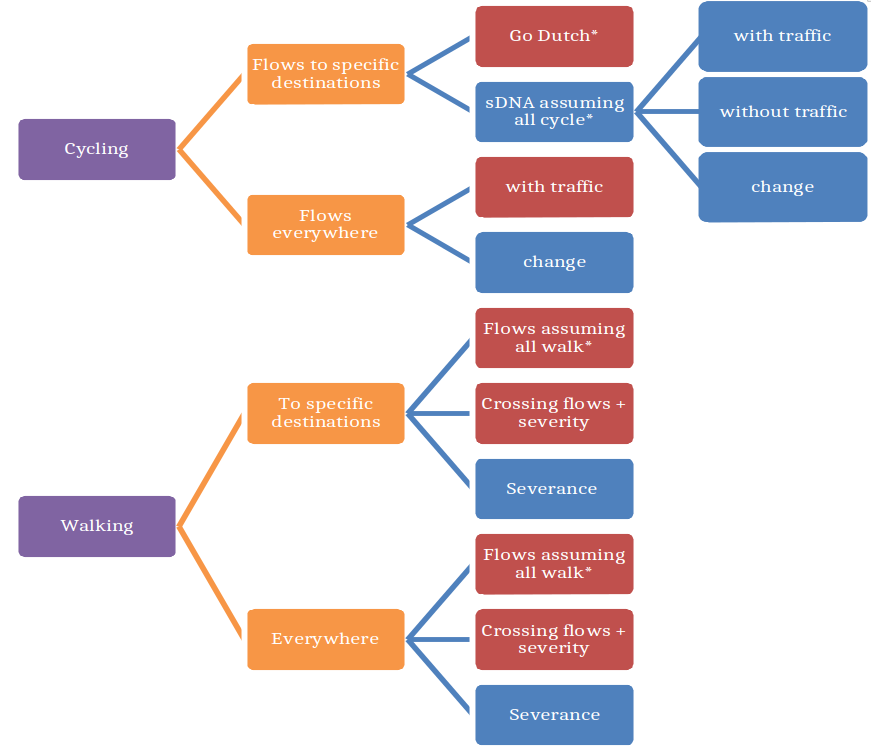
\includegraphics[width=0.6\linewidth]{figures/flowchart} 

}

\caption{Hierarchy of modelling outputs, with key layers (those included in walking/cycling summaries) shown in red.}\label{fig:flowchart}
\end{figure}

\hypertarget{cycling-models}{%
\subsection{Cycling models}\label{cycling-models}}

Cycling models are presented both from the PCT approach and via a SpNA approach. SpNA (spatial network analysis) is realized through use of the sDNA (spatial design network analysis) software (Crispin H. V. Cooper and Chiaradia 2020).
It should be noted that these two approaches each define `potential' differently:

-PCT Go Dutch views potential as an ideal/target scenario with no traffic, and where overall cycling levels match those in Holland
-sDNA models assume people cycle all trips under a threshold `perceived distance.' Presence/absence of motorized traffic has an impact on cyclist perception of distance, therefore comparing with- and without-traffic scenarios indicates locations where traffic-free cycling infrastructure may be beneficial. In the case of specific-destination flows, sDNA outputs indicate counts of people based on SD data. Conversely in the case of everywhere-to-everywhere flows, these are unscaled; the primary aim in their inclusion is to show integration with the wider network.

\hypertarget{modelling-cycling-potential-the-pct-approach}{%
\subsubsection{Modelling cycling potential: the PCT approach}\label{modelling-cycling-potential-the-pct-approach}}

Shows potential flows from student home postcodes to specific destinations under the Go Dutch scenario in the Propensity to Cycle Tool. These are quantified as potential counts of travellers, using calibration derived from \ldots{} {[}cite{]} {[}Robin to expand{]}

\hypertarget{sdna-cycling-models}{%
\subsubsection{sDNA cycling models}\label{sdna-cycling-models}}

sDNA cycling models are based on `perceived distance' computed as follows, based on Chan and Cooper (2019):

Where multipliers, calculated for each link in the network are given in Table \ref{tab:multipliers}, and change of direction penalty = 15 metres for every 90 degrees.
Cyclist perceived distance is always calculated for return trips to take account of opposite slopes on the return journey (what goes down must come up!).

\begin{table}
\caption{\label{tab:multipliers}Distance multipliers for different road classes and slopes in cycling model}

\centering
\begin{tabular}[t]{lr}
\toprule
Link slope & Distance multiplier\\
\midrule
<2\% & 1.0\\
2-4\% & 1.4\\
4-6\% & 2.2\\
>6\% & 4.2\\
\bottomrule
\end{tabular}
\centering
\begin{tabular}[t]{lr}
\toprule
Link road class & Distance multiplier\\
\midrule
Trunk & 3.85\\
Primary & 1.94\\
Secondary & 1.04\\
Tertiary & 1.03\\
Living/Residential & 0.95\\
\addlinespace
Traffic free & 0.95\\
\bottomrule
\end{tabular}
\end{table}

In the current models, sDNA cycling potential is based on the scenario where all return trips with perceived distance under 30km are cycled.
Note that with multipliers applied this translates to much shorter single trip distances in practice, e.g.~3-4 km on a trunk road, or a road with high gradient, but distances up to 15km under ideal conditions (a level, traffic free route).

For use of SD data, we employ sDNA's ability to import inter-zonal flow matrices. sDNA automatically distributes these over all links within each zone, rather than attaching them to zonal centroids, a known cause of inaccuracy in active travel models which must account for smaller scales than typical in vehicular models (Crispin H. V. Cooper 2017).
This process is complicated by the fact that some network links form the boundary between postcode zones and hence represent origins and destinations in more than one zone.
To resolve the issue, a one-to-many spatial join is carried out to assign zone labels to network links, i.e.~where links appear in multiple zones, they are duplicated for the purpose of analysis.
Following assignment of flows to links, a many-to-one database table join is conducted to aggregate flows from all links thus duplicated, into a single record for each link.

\hypertarget{walking-models-computed-by-spatial-network-analysis}{%
\subsection{Walking models computed by spatial network analysis}\label{walking-models-computed-by-spatial-network-analysis}}

sDNA walking propensity figures for specific destinations are based on the scenario that all trips under 3km are walked (at a brisk walking pace this is a journey of approximately 35 minutes, realistic for a commute to school).
Everywhere-to-everywhere flows use instead a cutoff of 1.5km as the majority of walking trips in this more general context will be shorter than this latter figure.

The barriers presented to pedestrian transport by the necessity of crossing major roads are well known, and typically referred to as severance, though this term can also refer to a number of different approaches to measuring the same phenomenon (James, Millington, and Tomlinson 2005; Mindell and Karlsen 2012; Quigley and Thornley 2011).
We choose to model this explicitly in pedestrian route choice in order to identify locations where crossing infrastructure can be improved.
The road network is thus pre-processed by a script which splits any road of tertiary, or higher, classification into two in order to model each side of the road separately.
Formal crossings are inserted wherever indicated by the network data, and informal crossings are inserted at all junctions (in reality pedestrians may cross anywhere along each link, but in the absence of data describing this, we do not model this detail: the difference in walking distance caused by exact crossing position is minimal in any case).

A route choice study in the town of Hereford (conveniently under 30km from our own study area, but taken to be representative of UK regional towns) Anciaes and Jones (2020) derived a revealed preference model of ``willingness to walk.''
In the current study these figures were translated to distance by assuming a walk speed of 4km/h; therefore we penalize crossings as follows (for the purpose of determining route choice, not whether or not the trip is walked):

\begin{enumerate}
\def\labelenumi{\arabic{enumi}.}
\tightlist
\item
  trunk, primary or secondary road, informal crossing: add 340 metres
\item
  tertiary road informal crossing: add 191 metres
\item
  any formal crossing: add 60 metres (As OSM data on crossing type was not found to be reliable at the time of the study, we take the average of signalized and refuge crossing coefficients to obtain this penalty.)
\end{enumerate}

In addition to predicting walking flows on both links and crossings, we also produce layers measuring severance by showing circuity --- the extra distance that must be walked to the destination from each point, compared to straight line distance.
This identifies areas which are cut off not only by major road crossings but also by physical barriers such as river, or railways, or urban layouts lacking in permeability. In the case of specific destinations, this is displayed as extra distance experienced by trips from each origin; in the case of everywhere-to-everywhere flows this is instead shown as a ratio of distances as the absolute distance must be interpreted in the context of each destination.

As with the cycling models, for specific-destination flows a one-to-many spatial join is carried out to assign zone labels to network links, and following the main analysis, a many-to-one table join to aggregate flows to a single record per link.

\hypertarget{automation}{%
\subsection{Automation}\label{automation}}

As mentioned in previous sections, there is demand for estimates of active travel potential down to the route network level in many places worldwide, and many places have access to data from which travel patterns to key destinations can be inferred.

To support the production of results in other areas, to enable reproducibility, and iteration on our results we developed an automated workflow.
We used a makefile, a build system which automatically determines which outputs need to be updated at any point, thus avoiding unnecessary repetition of computationally expensive models.

For data analysis and modelling we used R and Python.
Data analysis and geographic operations required for the Propensity to Cycle Tool used the packages \texttt{sf}, \texttt{stplanr}, and \texttt{osmdata} for geographic processing, routing and OSM data access, respectively (Lovelace and Ellison 2018; Padgham et al. 2017; Pebesma 2018)
The SNA approach, on the other hand, made use of the `Python stack,' including \texttt{GeoPandas}, \texttt{shapely} and \texttt{pyrosm} (Gillies and others 2007; Jordahl et al. 2020; Tenkanen 2020).

Network data is downloaded from OpenStreetMap based on a user-provided buffer polygon for the model area, using pyrosm (Tenkanen 2020).
A network processing step was scripted using QGIS (QGIS Development Team 2019) to snap downloaded pedestrian crossing points to the relevant nodes.
To allow greater flexibility we define our own rules (in the script \texttt{osm\_download.py}) for walking and cycling access to each network link.
We erred on the side of permissiveness in cases where OSM tagging data was ambiguous.
We also define here a `cyclist deterrence' field based on the OSM highway classification tag; this is a dummy motorized annual average daily traffic flow (measured in vehicles per hour) representative of each road class as defined in Chan and Cooper (2019), and is later used to determine the multipliers shown in table XX above.

The function \texttt{v.clean} from the GRASS GIS software (Neteler and Mitasova 2008) to break OSM polylines where they share nodes, thus converting the downloaded network to routable form complying with an endpoint connectivity rule.
sDNA Prepare is used to remove isolated systems and pseudonodes except where they are required to preserve different access, deterrence or splitting rules for subsections of links (Crispin H. V. Cooper and Chiaradia 2020); this greatly reduces the link count and hence computational load.
Metadata is automatically generated in json format alongside modelling outputs, based on the \texttt{view-metadata-template.jsontemplate} file.
We define hierarchy of ``views,'' each of which contain one or more data layers, complete with descriptions of the data and recommended symbology for display.
These are automatically processed to form:

\begin{enumerate}
\def\labelenumi{\arabic{enumi}.}
\tightlist
\item
  data dictionaries in HTML format
\item
  a web-based interactive map of outputs
\item
  QGIS project files containing all generated data displayed in the recommended manner, generated by the \texttt{create-qgis-project-from-metadata.py} script.
  The latter forms a useful starting point for users of the data to produce their own custom maps.
  Finally, following feedback from pracitioners, we created two summary output maps per town, one for cycling (Figure \ref{fig:sdnaresult}, left), and one for walking (Figure \ref{fig:sdnaresult}, right).
\end{enumerate}

These figures are generated using the \texttt{create-qgis-cycle-summary.py} and \texttt{create-qgis-walk-summary.py} scripts.

\begin{figure}

{\centering 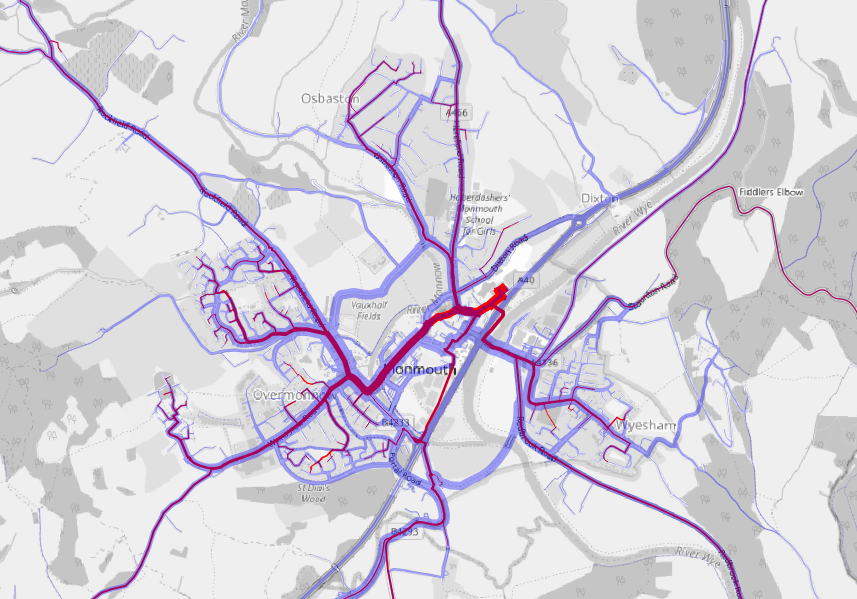
\includegraphics[width=0.49\linewidth]{figures/sdnaresult} 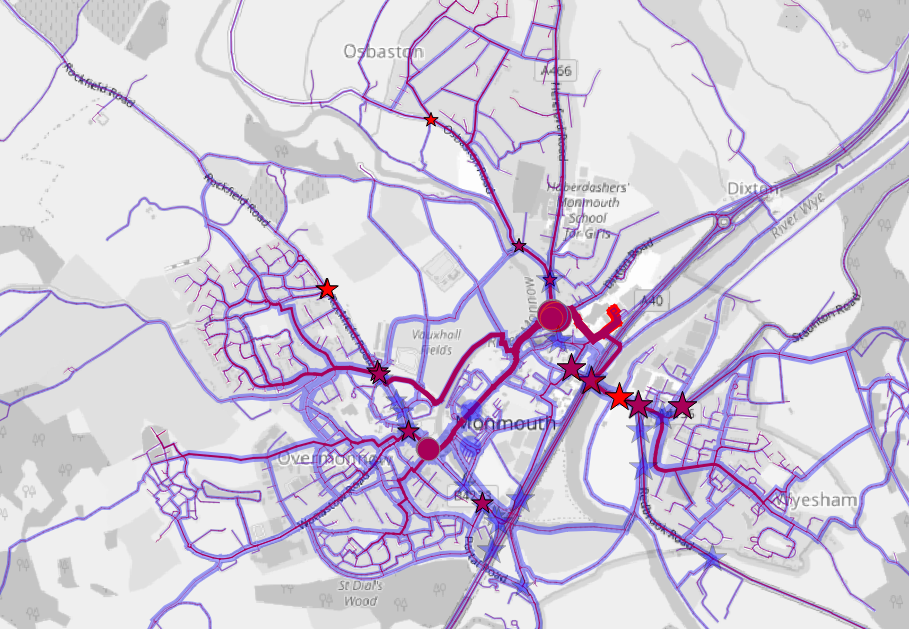
\includegraphics[width=0.49\linewidth]{figures/sdnaresult2} 

}

\caption{Cycling 'Go Dutch' scenario for Monmouth school (red) overlaid on unscaled everywhere-to-everywhere cycle flows (purple) to show the relationship of desirable routes to school (given suitable infrastructure) with the wider active travel network (left). Predicted walking flows to Monmouth school (red) overlaid on everywhere-to-everywhere flows (purple). Circles show formal road crossings; stars show informal crossings; size of crossing symbol indicates severity of road. Automated rendering thanks to QGIS, network data and background mapping © OpenStreetMap contributors.}\label{fig:sdnaresult}
\end{figure}

\hypertarget{references}{%
\section*{References}\label{references}}
\addcontentsline{toc}{section}{References}

\hypertarget{refs}{}
\begin{CSLReferences}{1}{0}
\leavevmode\hypertarget{ref-aguilera_passenger_2014}{}%
Aguiléra, Anne, and Jean Grébert. 2014. {``Passenger Transport Mode Share in Cities: Exploration of Actual and Future Trends with a Worldwide Survey.''} \emph{International Journal of Automotive Technology and Management} 14 (3-4): 203--16. \url{https://doi.org/10.1504/IJATM.2014.065290}.

\leavevmode\hypertarget{ref-ahmad_comparison_2020}{}%
Ahmad, Sohail, Anna Goodman, Felix Creutzig, James Woodcock, and Marko Tainio. 2020. {``A Comparison of the Health and Environmental Impacts of Increasing Urban Density Against Increasing Propensity to Walk and Cycle in {Nashville}, {USA}.''} \emph{Cities \& Health} 4 (1): 55--65. \url{https://doi.org/10.1080/23748834.2019.1659667}.

\leavevmode\hypertarget{ref-anciaes_comprehensive_2020}{}%
Anciaes, Paulo, and Peter Jones. 2020. {``A Comprehensive Approach for the Appraisal of the Barrier Effect of Roads on Pedestrians.''} \emph{Transportation Research Part A: Policy and Practice} 134 (April): 227--50. \url{https://doi.org/10.1016/j.tra.2020.02.003}.

\leavevmode\hypertarget{ref-aoun_bicycle_2015}{}%
Aoun, A. 2015. \emph{Bicycle and Pedestrian Forecasting Tools: {State} of the Practice}. {NC}: {Chapel Hill}.

\leavevmode\hypertarget{ref-beecham_visual_2012}{}%
Beecham, Roger, Jo Wood, and Audrey Bowerman. 2012. {``A Visual Analytics Approach to Understanding Cycling Behaviour.''} In \emph{2012 {IEEE Conference} on {Visual Analytics Science} and {Technology} ({VAST})}, 207--8. {IEEE}.

\leavevmode\hypertarget{ref-boyce_forecasting_2015}{}%
Boyce, David E., and Huw C. W. L. Williams. 2015. \emph{Forecasting {Urban Travel}: {Past}, {Present} and {Future}}. {Edward Elgar Publishing}.

\leavevmode\hypertarget{ref-cervero_travel_1997}{}%
Cervero, Robert, and Kara Kockelman. 1997. {``Travel Demand and the {3Ds}: {Density}, Diversity, and Design.''} \emph{Transportation Research Part D: Transport and Environment} 2 (3): 199--219. \url{https://doi.org/10.1016/S1361-9209(97)00009-6}.

\leavevmode\hypertarget{ref-chan_using_2019}{}%
Chan, Eric Yin Cheung, and Crispin HV Cooper. 2019. {``Using Road Class as a Replacement for Predicted Motorized Traffic Flow in Spatial Network Models of Cycling.''} \emph{Scientific Reports} 9 (1): 1--12.

\leavevmode\hypertarget{ref-cooper_using_2019}{}%
Cooper, C. H. V., Ian Harvey, Scott Orford, and Alain J. F. Chiaradia. 2019. {``Using Multiple Hybrid Spatial Design Network Analysis to Predict Longitudinal Effect of a Major City Centre Redevelopment on Pedestrian Flows.''} \emph{Transportation}, December. \url{https://doi.org/10.1007/s11116-019-10072-0}.

\leavevmode\hypertarget{ref-cooper_using_2017}{}%
Cooper, Crispin H. V. 2017. {``Using Spatial Network Analysis to Model Pedal Cycle Flows, Risk and Mode Choice.''} \emph{Journal of Transport Geography} 58 (January): 157--65. \url{https://doi.org/10.1016/j.jtrangeo.2016.12.003}.

\leavevmode\hypertarget{ref-cooper_predictive_2018}{}%
---------. 2018. {``Predictive Spatial Network Analysis for High-Resolution Transport Modeling, Applied to Cyclist Flows, Mode Choice, and Targeting Investment.''} \emph{International Journal of Sustainable Transportation} 0 (0): 1--11. \url{https://doi.org/10.1080/15568318.2018.1432730}.

\leavevmode\hypertarget{ref-cooper_sdna_2020}{}%
Cooper, Crispin H. V., and Alain J. F. Chiaradia. 2020. {``{sDNA}: 3-d Spatial Network Analysis for {GIS}, {CAD}, {Command Line} \& {Python}.''} \emph{SoftwareX} 12 (July): 100525. \url{https://doi.org/10.1016/j.softx.2020.100525}.

\leavevmode\hypertarget{ref-cooper_cycletopia_2017}{}%
Cooper, Jai, and Terry Leahy. 2017. {``Cycletopia in the Sticks: Bicycle Advocacy Beyond the City Limits.''} \emph{Mobilities}, January, 1--17. \url{https://doi.org/10.1080/17450101.2016.1254898}.

\leavevmode\hypertarget{ref-ewing_varying_2014}{}%
Ewing, Reid, Guang Tian, J. P. Goates, Ming Zhang, Michael J. Greenwald, Alex Joyce, John Kircher, and William Greene. 2014. {``Varying Influences of the Built Environment on Household Travel in 15 Diverse Regions of the {United States}.''} \emph{Urban Studies} 52 (13): 2330--48. \url{https://doi.org/10.1177/0042098014560991}.

\leavevmode\hypertarget{ref-forsyth_urban_2011}{}%
Forsyth, Ann, and Kevin Krizek. 2011. {``Urban Design: Is There a Distinctive View from the Bicycle?''} \emph{Journal of Urban Design} 16 (4): 531--49.

\leavevmode\hypertarget{ref-frank_impacts_1994}{}%
Frank, Lawrence D., and Gary Pivo. 1994. {``Impacts of Mixed Use and Density on Utilization of Three Modes of Travel: {Single}-Occupant Vehicle, Transit, Walking.''} \emph{Transportation Research Record}, no. 1466. \url{https://trid.trb.org/view/425321}.

\leavevmode\hypertarget{ref-gillies_shapely_2007}{}%
Gillies, Sean, and others. 2007. \emph{Shapely: Manipulation and Analysis of Geometric Objects}. {toblerity.org}. \url{https://github.com/Toblerity/Shapely}.

\leavevmode\hypertarget{ref-goodman_scenarios_2019}{}%
Goodman, Anna, Ilan Fridman Rojas, James Woodcock, Rachel Aldred, Nikolai Berkoff, Malcolm Morgan, Ali Abbas, and Robin Lovelace. 2019. {``Scenarios of Cycling to School in {England}, and Associated Health and Carbon Impacts: {Application} of the {`{Propensity} to {Cycle Tool}'}.''} \emph{Journal of Transport \& Health} 12 (March): 263--78. \url{https://doi.org/10.1016/j.jth.2019.01.008}.

\leavevmode\hypertarget{ref-gotschi_comprehensive_2017}{}%
Götschi, Thomas, Audrey de Nazelle, Christian Brand, Regine Gerike, and Regine Gerike. 2017. {``Towards a {Comprehensive Conceptual Framework} of {Active Travel Behavior}: A {Review} and {Synthesis} of {Published Frameworks}.''} \emph{Current Environmental Health Reports} 4 (3): 286--95. \url{https://doi.org/10.1007/s40572-017-0149-9}.

\leavevmode\hypertarget{ref-grise_if_2018}{}%
Grisé, Emily, and Ahmed El-Geneidy. 2018. {``If We Build It, Who Will Benefit? {A} Multi-Criteria Approach for the Prioritization of New Bicycle Lanes in {Quebec City}, {Canada}.''} \emph{Journal of Transport and Land Use} 11 (1). \url{https://doi.org/10.5198/jtlu.2018.1115}.

\leavevmode\hypertarget{ref-griswold_pedestrian_2019}{}%
Griswold, Julia B., Aditya Medury, Robert J. Schneider, Dave Amos, Ang Li, and Offer Grembek. 2019. {``A Pedestrian Exposure Model for the California State Highway System.''} \emph{Transportation Research Record}, April, 0361198119837235. \url{https://doi.org/10.1177/0361198119837235}.

\leavevmode\hypertarget{ref-handy_critical_2005}{}%
Handy, Susan L. 2005. \emph{Critical Assessment of the Literature on the Relationships Among Transportation, Land Use, and Physical Activity}. Transportation Research Board and the Institute of Medicine Committee on Physical Activity, Health, Transportation, and Land Use 282. {Resource paper for TRB Special Report}.

\leavevmode\hypertarget{ref-handy_how_2002}{}%
Handy, Susan L., Marlon G. Boarnet, Reid Ewing, and Richard E. Killingsworth. 2002. {``How the Built Environment Affects Physical Activity: Views from Urban Planning.''} \emph{American Journal of Preventive Medicine} 23 (August): 64--73.

\leavevmode\hypertarget{ref-handy_promoting_2014}{}%
Handy, Susan, Bert van Wee, and Maarten Kroesen. 2014. {``Promoting {Cycling} for {Transport}: {Research Needs} and {Challenges}.''} \emph{Transport Reviews} 34 (1): 4--24. \url{https://doi.org/10.1080/01441647.2013.860204}.

\leavevmode\hypertarget{ref-hollander_transport_2016}{}%
Hollander, Yaron. 2016. \emph{Transport {Modelling} for a {Complete Beginner}}. {CTthink!}

\leavevmode\hypertarget{ref-james_understanding_2005}{}%
James, Emma, Anna Millington, and Paul Tomlinson. 2005. \emph{Understanding Community Severance Part {I} - Views of Practitioners and Communities}. {UK}: {Department for Transport}. \url{http://webarchive.nationalarchives.gov.uk/+/http:/www.dft.gov.uk/adobepdf/163944/Understanding_Community_Sev1.pdf}.

\leavevmode\hypertarget{ref-jordahl_geopandas_2020}{}%
Jordahl, K., Wasserman J. Van den Bossche Joris, J. McBride, M. Fleischmann, J. Gerard, J. Tratner, M. Perry, C. Farmer, G. A. Hjelle, and S. Gillies. 2020. \emph{Geopandas/Geopandas: {V0}. 7.0. {Zenodo}}.

\leavevmode\hypertarget{ref-kuzmyak_estimating_2014}{}%
Kuzmyak, J. Richard, Jerry Walters, Mark Bradley, and KM Kockelman. 2014. \emph{Estimating Bicycling and Walking for Planning and Project Development}. Nchrp National Cooperative Highway Research Program Report 770. {Washington, DC}: {Transportation Research Board of the National Academies}.

\leavevmode\hypertarget{ref-larouche_built_2015}{}%
Larouche, Richard. 2015. {``Built {Environment Features} That {Promote Cycling} in {School}-{Aged Children}.''} \emph{Current Obesity Reports} 4 (4): 494--503. \url{https://doi.org/10.1007/s13679-015-0181-8}.

\leavevmode\hypertarget{ref-larsen_build_2013}{}%
Larsen, Jacob, Zachary Patterson, and Ahmed El-Geneidy. 2013. {``Build It. {But} Where? {The} Use of Geographic Information Systems in Identifying Locations for New Cycling Infrastructure.''} \emph{International Journal of Sustainable Transportation} 7 (4): 299--317. \url{http://www.tandfonline.com/doi/abs/10.1080/15568318.2011.631098}.

\leavevmode\hypertarget{ref-lovelace_stplanr_2018}{}%
Lovelace, Robin, and Richard Ellison. 2018. {``Stplanr: {A Package} for {Transport Planning}.''} \emph{The R Journal} 10 (2): 7--23. \url{https://doi.org/10.32614/RJ-2018-053}.

\leavevmode\hypertarget{ref-lovelace_propensity_2017}{}%
Lovelace, Robin, Anna Goodman, Rachel Aldred, Nikolai Berkoff, Ali Abbas, and James Woodcock. 2017. {``The {Propensity} to {Cycle Tool}: {An} Open Source Online System for Sustainable Transport Planning.''} \emph{Journal of Transport and Land Use} 10 (1). \url{https://doi.org/10.5198/jtlu.2016.862}.

\leavevmode\hypertarget{ref-lovelace_open_2020}{}%
Lovelace, Robin, John Parkin, and Tom Cohen. 2020. {``Open Access Transport Models: {A} Leverage Point in Sustainable Transport Planning.''} \emph{Transport Policy} 97 (October): 47--54. \url{https://doi.org/10.1016/j.tranpol.2020.06.015}.

\leavevmode\hypertarget{ref-lovelace_methods_2020}{}%
Lovelace, Robin, Joseph Talbot, Malcolm Morgan, and Martin Lucas-Smith. 2020. {``Methods to {Prioritise Pop}-up {Active Transport Infrastructure}.''} \emph{Transport Findings}, July, 13421. \url{https://doi.org/10.32866/001c.13421}.

\leavevmode\hypertarget{ref-martinez-gil_modeling_2017}{}%
Martinez-Gil, F., M.-F.I. Lozano, and F. Fernández. 2017. {``Modeling, Evaluation, and Scale on Artificial Pedestrians: A Literature Review.''} \emph{ACM Computing Surveys (CSUR)} 50 (5): p.72..

\leavevmode\hypertarget{ref-mccormack_search_2011}{}%
McCormack, Gavin R., and Alan Shiell. 2011. {``In Search of Causality: A Systematic Review of the Relationship Between the Built Environment and Physical Activity Among Adults.''} \emph{International Journal of Behavioral Nutrition and Physical Activity} 8 (1): 1--11.

\leavevmode\hypertarget{ref-mindell_community_2012}{}%
Mindell, Jennifer S, and Saffron Karlsen. 2012. {``Community Severance and Health: What Do We Actually Know?''} \emph{Journal of Urban Health: Bulletin of the New York Academy of Medicine} 89 (2): 232--46. \url{https://doi.org/10.1007/s11524-011-9637-7}.

\leavevmode\hypertarget{ref-munira_use_2017}{}%
Munira, S., and I. N. Sener. 2017. \emph{Use of the Direct-Demand Modeling in Estimating Nonmotorized Activity: {A} Meta-Analysis. {Technical} Report Prepared for the Safety Through Disruption (Safe-d)}. {TX: National University Transportation Center. Texas A\&M Transportation Institute}.

\leavevmode\hypertarget{ref-neteler_open_2008}{}%
Neteler, Markus, and Helena Mitasova. 2008. \emph{Open Source {GIS}: A {GRASS GIS} Approach}. 3. ed. {New York, NY}: {Springer}.

\leavevmode\hypertarget{ref-padgham_osmdata_2017}{}%
Padgham, Mark, Robin Lovelace, Maëlle Salmon, and Bob Rudis. 2017. {``Osmdata.''} \emph{The Journal of Open Source Software} 2 (14). \url{https://doi.org/10.21105/joss.00305}.

\leavevmode\hypertarget{ref-pebesma_simple_2018}{}%
Pebesma, Edzer. 2018. {``Simple {Features} for {R}: {Standardized Support} for {Spatial Vector Data}.''} \emph{The R Journal}. \url{https://journal.r-project.org/archive/2018/RJ-2018-009/index.html}.

\leavevmode\hypertarget{ref-pucher_walking_2010}{}%
Pucher, John, Ralph Buehler, David R. Bassett, and Andrew L. Dannenberg. 2010. {``Walking and Cycling to Health: {A} Comparative Analysis of City, State, and International Data.''} \emph{American Journal of Public Health} 100 (10): 1986--92. \url{https://doi.org/10.2105/AJPH.2009.189324}.

\leavevmode\hypertarget{ref-qgisdevelopmentteam_qgis_2019}{}%
QGIS Development Team. 2019. \emph{{QGIS Geographic Information System}}. {Open Source Geospatial Foundation}. \url{http://qgis.osgeo.org}.

\leavevmode\hypertarget{ref-quigley_literature_2011}{}%
Quigley, R, and L Thornley. 2011. \emph{Literature Review on Community Cohesion and Community Severance: {Definitions} and Indicators for Transport Planning and Monitoring}. {Wellington}: {Quigley and Watts Ltd}. \url{http://www.nzta.govt.nz/resources/community-cohesion-and-community-severance/docs/community-cohesion-and-community-severance.pdf}.

\leavevmode\hypertarget{ref-raffler_cycling_2019}{}%
Raffler, Clemens, Tadej Brezina, and Günter Emberger. 2019. {``Cycling Investment Expedience: {Energy} Expenditure Based {Cost}-{Path Analysis} of National Census Bicycle Commuting Data.''} \emph{Transportation Research Part A: Policy and Practice} 121 (March): 360--73. \url{https://doi.org/10.1016/j.tra.2019.01.019}.

\leavevmode\hypertarget{ref-tatem_worldpop_2017}{}%
Tatem, Andrew J. 2017. {``{WorldPop}, Open Data for Spatial Demography.''} \emph{Scientific Data} 4 (January): 170004. \url{https://doi.org/10.1038/sdata.2017.4}.

\leavevmode\hypertarget{ref-tenkanen_pyrosm_2020}{}%
Tenkanen, Henrikki. 2020. \emph{Pyrosm} (version v0.6.0 (Nov 18, 2020)). \url{https://pyrosm.readthedocs.io/en/latest/}.

\leavevmode\hypertarget{ref-turner_synthesis_2017}{}%
Turner, S. 2017. \emph{Synthesis of Methods for Estimating Pedestrian and Bicyclist Exposure to Risk at Area Wide Levels and on Specific Transportation Facilities}. {Washington, DC}: {Federal Highway Administration. Office of Safety}.

\leavevmode\hypertarget{ref-uttley_cycling_2016}{}%
Uttley, J., and R. Lovelace. 2016. {``Cycling Promotion Schemes and Long-Term Behavioural Change: {A} Case Study from the {University} of {Sheffield}.''} \emph{Case Studies on Transport Policy} 4 (2). \url{https://doi.org/10.1016/j.cstp.2016.01.001}.

\leavevmode\hypertarget{ref-welshgovernment_active_2020}{}%
Welsh Government. 2020. {``Active {Travel Guidance}.''} {Welsh Government}. \url{https://gov.wales/sites/default/files/consultations/2020-02/active-travel-guidance_1.pdf}.

\leavevmode\hypertarget{ref-zhang_prioritizing_2014}{}%
Zhang, Dapeng, David Jose Ahouagi Vaz Magalhaes, and Xiaokun (Cara) Wang. 2014. {``Prioritizing Bicycle Paths in {Belo Horizonte City}, {Brazil}: {Analysis} Based on User Preferences and Willingness Considering Individual Heterogeneity.''} \emph{Transportation Research Part A: Policy and Practice} 67: 268--78. \url{https://doi.org/10.1016/j.tra.2014.07.010}.

\end{CSLReferences}

% \section{Introduction}
%
%
%
%
%
% \section{Section name}
% \label{sec:section-name}
%
%
%
% \subsection{Subsection heading}


%%%%%%%%%%
% \begin{figure*}[htbp]
%   \centering
%   \includegraphics{fig1}
%   \caption{Caption ...  }
%   \label{fig:1}
% \end{figure*}



\bibliographystyle{jtlu}
\bibliography{../Bib/filename}

\end{document}
